% Drawing 67/01-1 -- folder 67, batch 01, archive page 2 (PDF page 3).
% Transcription: à gauche, un croquis de $\widetilde{X}$ : deux anneaux hachurés le long de deux composantes du bord, l'épaisseur de chacun marquée $\varepsilon_{i}$, et sous le dessin « $0 \leqslant \varepsilon_{i} < +\infty$ »
% Kind: surface with collars (annuli along boundary components). Method 2 (schematic redraw from the facsimile). Status: ok.
% Notes: Two rings (annuli along two boundary components), each with hatching on part of the collar and a small epsilon_i marking its width; under them "0 <= epsilon_i < +infinity". The long faint ruled-looking strokes crossing the crop belong to the writing of the page and are left out, as is a small struck sign above the right ring.
% Coordinates: 1 unit = 1 mm = 1/100 of the crop width (bbox in page fractions: [0.12, 0.5, 0.52, 0.66]).
% Redrawn by Claude (claude-opus-5-5), issue #73, 2026-11-07; not checked by a human; not compiled (no TeX in the session).
% Rights: reproduces part of the work -- behind RENDER_TRANSCRIPTS, never published by itself.
\documentclass[tikz,border=3pt]{standalone}
\usepackage{amsmath,amssymb}
\usetikzlibrary{patterns,arrows.meta}
\tikzset{pencil/.style={black!45}, struck/.style={black!35}, mark/.style={circle,draw,inner sep=1.3pt}, pt/.style={circle,fill,inner sep=0.9pt}, opt/.style={circle,draw,fill=white,inner sep=1.1pt}}
\begin{document}
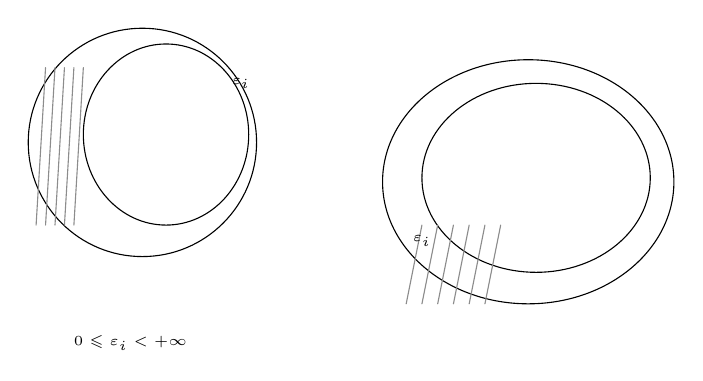
\begin{tikzpicture}[x=1mm,y=1mm,line cap=round,line join=round,font=\scriptsize]
\draw (26.5,-33.5) ellipse[x radius=14.5, y radius=14.5];
\draw (29.5,-32.5) ellipse[x radius=10.5, y radius=11.5];
\draw[pencil] (13,-44) -- (14.2,-24);
\draw[pencil] (14.2,-44) -- (15.4,-24);
\draw[pencil] (15.4,-44) -- (16.6,-24);
\draw[pencil] (16.6,-44) -- (17.8,-24);
\draw[pencil] (17.8,-44) -- (19,-24);
\draw (75.5,-38.5) ellipse[x radius=18.5, y radius=15.5];
\draw (76.5,-38) ellipse[x radius=14.5, y radius=12];
\draw[pencil] (60,-54) -- (62,-44);
\draw[pencil] (62,-54) -- (64,-44);
\draw[pencil] (64,-54) -- (66,-44);
\draw[pencil] (66,-54) -- (68,-44);
\draw[pencil] (68,-54) -- (70,-44);
\draw[pencil] (70,-54) -- (72,-44);
\node[inner sep=1pt] at (39,-26) {\tiny $\varepsilon_i$};
\node[inner sep=1pt] at (62,-46) {\tiny $\varepsilon_i$};
\node[inner sep=1pt] at (25,-59) {\tiny $0\leqslant\varepsilon_i<+\infty$};
\end{tikzpicture}
\end{document}
